\section{Near-field sensor post-processing}
\label{sec:on-chip-near-field-process}

%TODO Introduction to near-field current processing

% Introduction
In this section, two different methods are described for reconstructing the original current from a near-field magnetic scanner measurement.
Each method requires a characterization of the sensor, to obtain its transfer function.
Overall, they differ mostly in the modelisation of the transfer function.
The original time-domain waveform is obtained by using the measured waveform and the inverse transfer function.
%TODO: Refs monnereau, review of nfs methods

\subsection{Physical concepts}
\label{sec:phys-concepts-nfs}

The sensor is a near-field magnetic current loop.
We are interested in the relation between voltage difference across the sensor and the current value circulating through the track.

% Creation of the magnetic field
Circulating current in a conductor creates a magnetic field.
In steady-state conditions (static current), and by approximating the shape of the metal track to an infinitely long wire, Biot-savart law could be employed (Eq. \ref{eq:biot-savart}).
It states that magnetic field decreases with the square of the distance from a current segment of the track.
\begin{equation}
  \label{eq:biot-savart}
  \overrightarrow{B}(\overrightarrow{r}) = \frac{\mu_{0}}{4\pi}\oint_{C}\frac{I \mathrm{d}\overrightarrow{l} \wedge (\overrightarrow{r} - \overrightarrow{r'}) }{|\overrightarrow{r} - \overrightarrow{r'}|^3}
\end{equation}

However Biot-Savart works only for magnetostatic approximation ? What is it ?
Steady state magnetic field.
General purpose is Jefimenko's equations

% Generation of voltage difference from the magnetic
The sensor is placed near the monitored metal track.
The sensor is approximated as a perfect loop in a magnetic field.
In that case, the Faraday law's of induction gives Eq. \ref{eq:faraday}
where \textepsilon{} is the electromotrice force (TODO: gloss) and \textPhi{}\textsubscript{B} is given in \ref{eq:phi}.

\begin{equation} \label{eq:faraday}
  \varepsilon = - \frac{\mathrm{d} \phi _{B}}{\mathrm{d} t}
\end{equation}


\textPhi{}\textsubscript{B} is the magnetic flux through the loop, $B$ is the magnetic field, \textSigma{}(t) is a surface bounded by the closed contour,
and $dA$ is an infinitesimal vector area element of \textSigma{}(t) (magnitude is the area of the element, direction is orthogonal to the loop surface).

\begin{equation} \label{eq:phi}
  \phi _{B} = - \iint_{\Sigma(t)} \mathrm{d}A . B(r,t)
\end{equation}

% Global equation and conclusion
%TODO: eq
Original current and measured voltage are related by a time-domain derivative ? Only in magnetostatic conditions ?

\subsection{Time-domain integration method}

% Describe the algorithm
As detailed previously in \ref{sec:phys-concepts-nfs}, the measured voltage is proportional to the time derivative of the original current.
The time-domain method is based on this property.
The original current waveform is the integral of the sensor voltage times a scale factor plus an offset.
The offset and scale factor can be determined experimentally with the calibration.

% Talk about calibration
The calibration is conducted with the calibration sensor integrated on silicon (\ref{fig:calibration-sensor}).
A square impulse is injected between pins S1 and S2, and the response is measured with a 2GHz bandwith 10GS/s oscilloscope in differential input between C1 and C2.
Both the injected current and measured voltage waveforms are recorded.

\begin{figure}[!h]
  \centering
  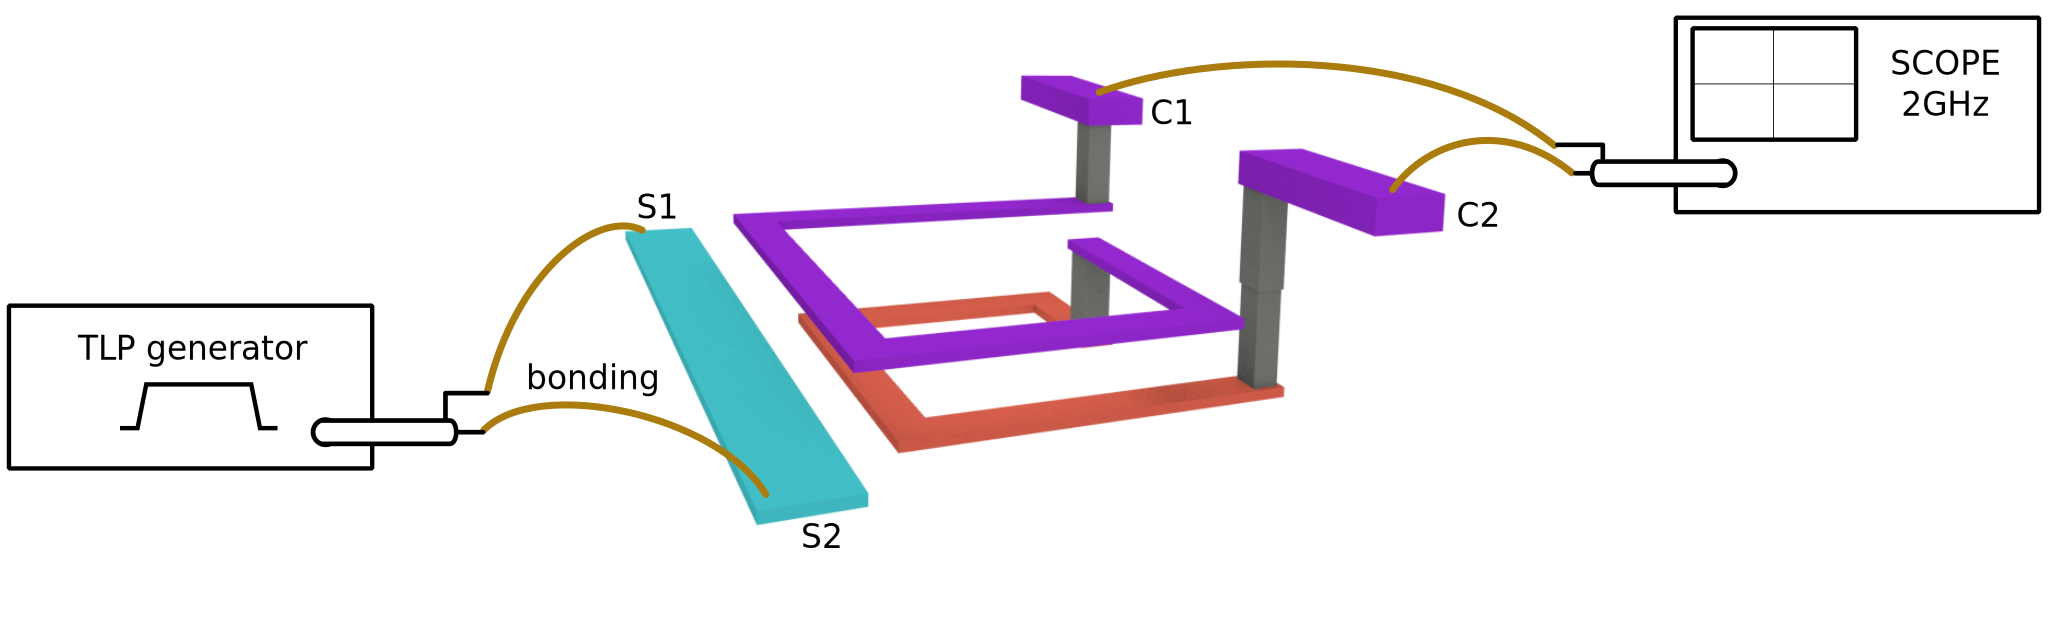
\includegraphics[width=0.9\textwidth]{src/3/figures/sensor_measurement_setup.pdf}
  \caption{Calibration sensor setup for time-domain method}
  \label{fig:calibration-sensor}
\end{figure}

% Integration method
Afterwards, the measured voltage is integrated with a trapezoidal method.
Experimentally, the correction factor with the current design was found to be $8.10^8$.
As a result of the integration, an offset is present.
The offset is calculated such as $V(t=0) = 0.$

The voltage waveform measured with the sensor is given Fig. \ref{fig:measurement-nfs}.
The reconstructed curve is compared to the original in Fig. \ref{fig:time-domain-reconstructed}.

\begin{figure}[!h]
  \centering
  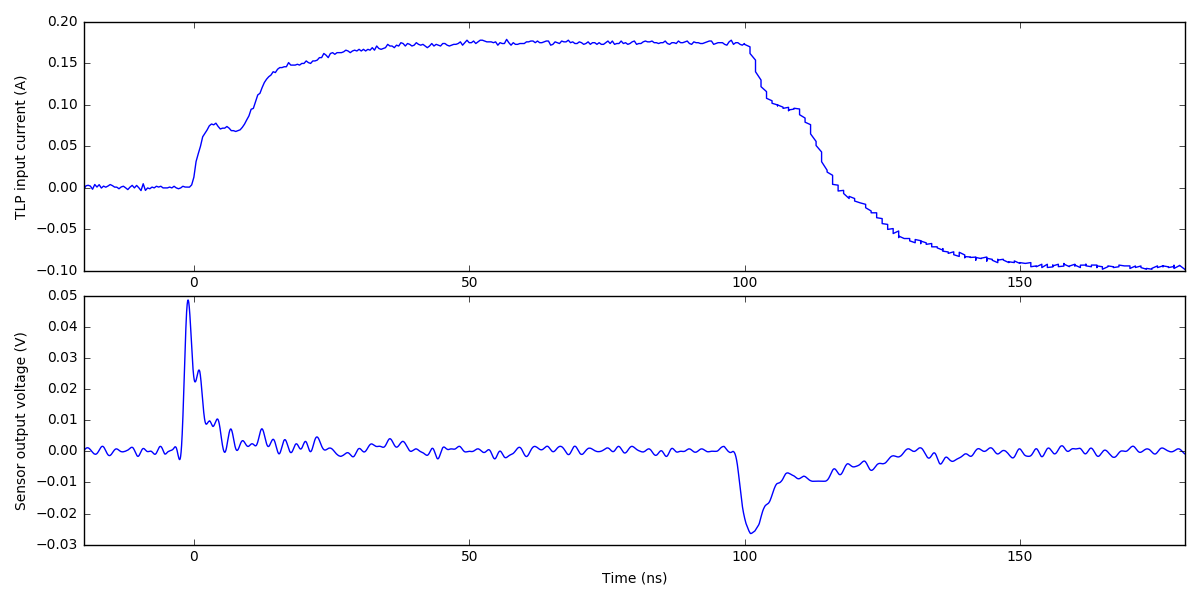
\includegraphics[width=0.9\textwidth]{src/3/figures/measured_waveform.png}
  \caption{Measured voltage waveform}
  \label{fig:measurement-nfs}
\end{figure}

%TODO: Comment : Curve is really derivative of a rectangular pulse

\begin{figure}[!h]
  \centering
  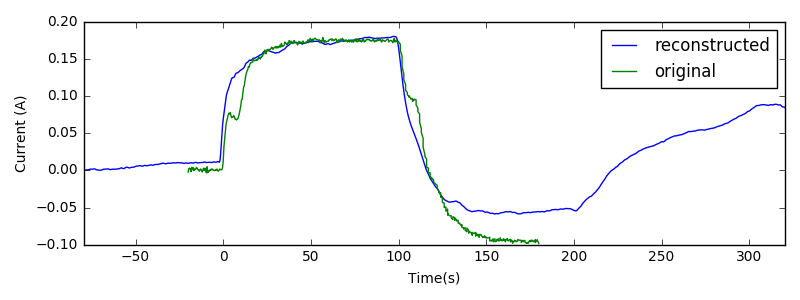
\includegraphics[width=0.9\textwidth]{src/3/figures/time_domain_vs_ref.png}
  \caption{Reference current waveform versus time-domain reconstructed}
  \label{fig:time-domain-reconstructed}
\end{figure}

% Limitations
For this particular rectangular pulse, the integration method seems to work well.
%TODO: test for more dynamic pulse.

% Defaults to overcome
The time-domain method is simple to compute.
However, it makes several approximations regarding the sensor's shape and the validity of the applicable physical laws.
Overall, it assumes that the gain of the sensor is constant for all frequencies, which is not correct either.

\subsection{Frequency-domain reconstruction method}
%TODO: Make a schematic to show the entire algorithm ?
% Intro
The frequency domain tries to improve the post-processing by taking the sensor's response into account.
More generally, this method applies to all types of sensors.
After characterization, the frequency response of the sensor is used to recompute the current time-domain waveform from the measured voltage time-domain waveform.

% Characterization
The characterization is conducted with the calibration sensor, using a \gls{vna}.
The calibration setup is given with in Fig. \ref{fig:calibration-sensor-rf}.

\begin{figure}[!h]
  \centering
  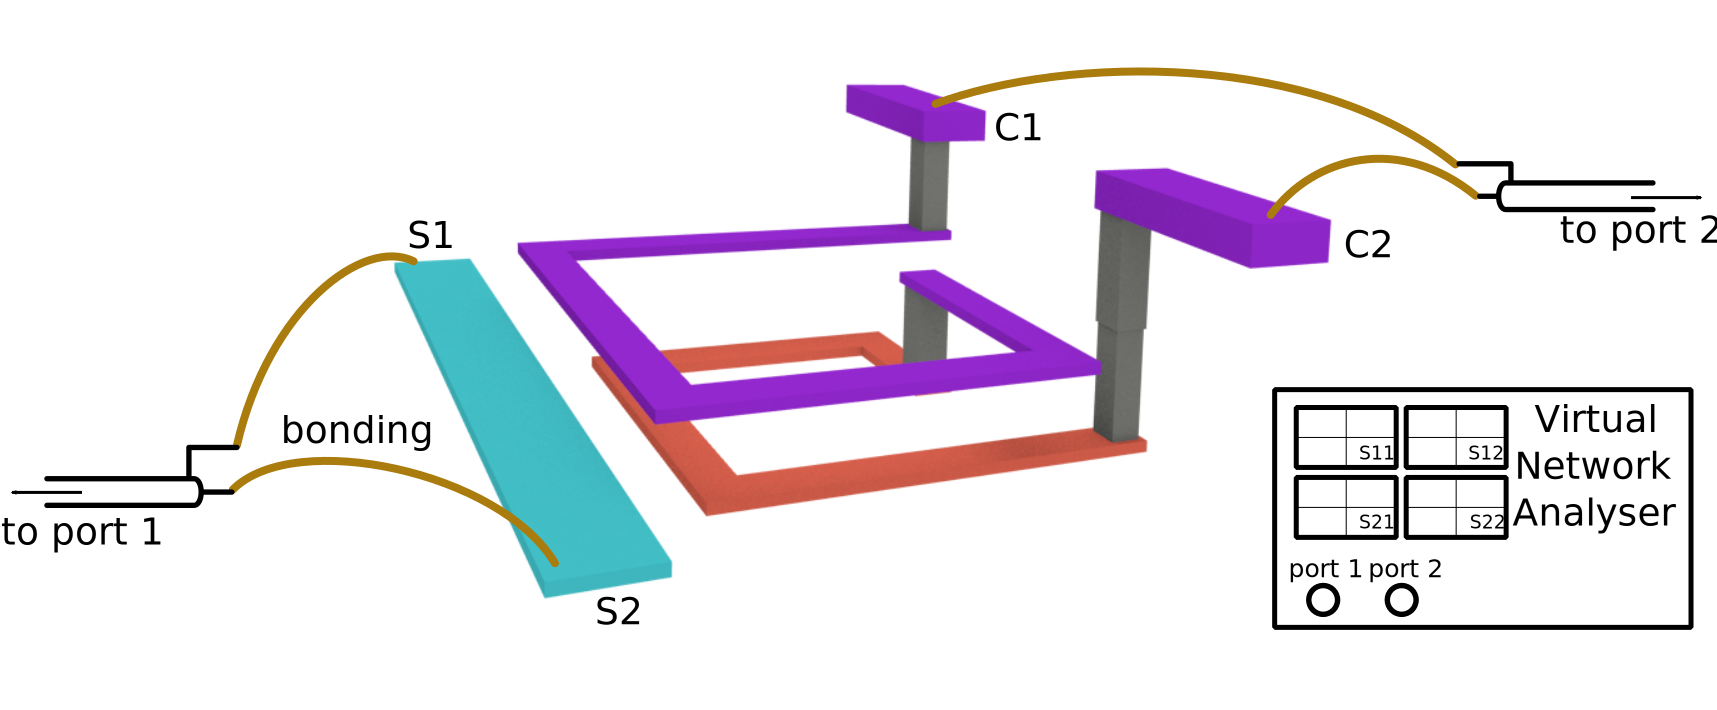
\includegraphics[width=0.9\textwidth]{src/3/figures/sensor_measurement_setup_rf.pdf}
  \caption{Calibration sensor setup for time-domain method}
  \label{fig:calibration-sensor-rf}
\end{figure}

% Detail characterization
The \gls{sparams} measurement of the sensor is given in Fig. \ref{fig:sensor-response}.
S11 is the reflected power at port 1.
S21 is the transmitted power between port 1 and port 2.
In theory, S12 is identical to S21 for symetrical 2-port devices.
And S22 is the reflected power from the output, which is not relevant for this study.

\begin{figure}[!h]
  \centering
  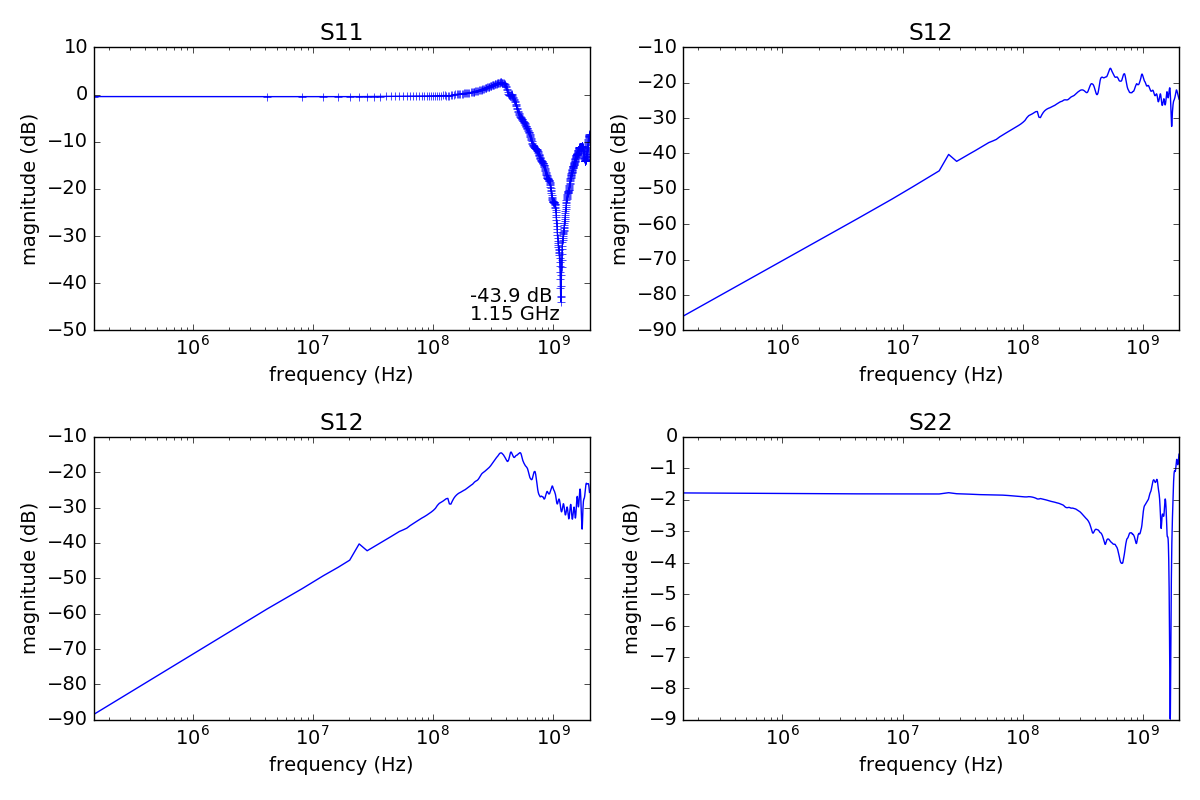
\includegraphics[width=0.9\textwidth]{src/3/figures/sensor_freq_response.png}
  \caption{Sensor frequency response}
  \label{fig:sensor-response}
\end{figure}

% Talk about S11
S11 shows a resonance of -43.9 dB at 1.15 GHz.
At this frequency, the maximum amount of power is transmitted between the metal track (port 1) and the sensor output (port 2).
As a consequence, the reflected power at port 1 is at its minimum value.

% Talk about S21
S21 is the only scattering parameter required by the post-processing method.
It represents the transfer function between the input current and the sensed voltage.
Previously, only the magnitude measurements were displayed in Fig. \ref{fig:sensor-response}.
However, the post-processing method aims at reconstuting a time-domain waveform, with a step inside the frequency domain.
With only the magnitude, the phase information is lost, making the reconstruction of the original signal impossible.
%TODO: Is it required to explain ? Make an example with a square impulse without phase information
Another \gls{sparams} measurement has been performed, configured to obtain both magnitude and phase information (Fig. \ref{fig:s21-response-complex}).

\begin{figure}[!h]
  \centering
  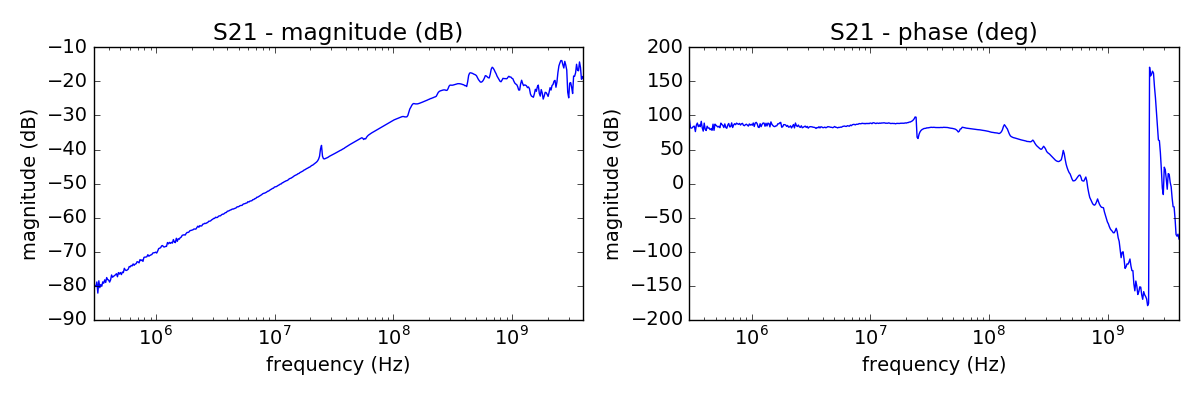
\includegraphics[width=0.9\textwidth]{src/3/figures/s21_freq_response.png}
  \caption{Sensor frequency response - complex S21 (magnitude and phase)}
  \label{fig:s21-response-complex}
\end{figure}

% Overall
It was suspected previously that the sensor's response is not constant versus frequency.
The \gls{sparams} measurement confirms it, and shows that the integration method is neglecting this variation.
Ideally, the goal is to measure with the largest bandwidth possible.
The S21 respone is used during post-processing to compensate this variation.

% The algorithm
The post-processing methods starts with computing the \gls{fft} of the voltage waveform, storing it in array \textit{fft\_measure}.
This array has the structure given in Table \ref{tab:complex-fft}.

\begin{table}[!h]
  \centering
  \begin{tabular}{@{}lllll@{}}
  \toprule
  frequencies (Hz)        & complex value                \\ \midrule
  1.0*10^6                & 0.33 + i0.2                  \\
  2.0*10^6                & 0.46 - i1.2                  \\
  etc.                    & etc.                         \\ \bottomrule
  \end{tabular}
  \caption{Structure for the result of (complex) FFT}
  \label{tab:complex-fft}
\end{table}

On the other hand, the S21 measurement, stored in array \textit{s21\_sensor}, has the structure of Table \ref{tab:sparams}.

\begin{table}[!h]
  \centering
  \begin{tabular}{@{}lllll@{}}
  \toprule
  frequencies (Hz)          & magnitude (dB)         & phase (rad)     \\ \midrule
  1.5*10^6                  & -10                    & 1.23            \\
  2.5*10^6                  & -12                    & 0.12            \\
  etc.                      & etc.                   & etc             \\ \bottomrule
  \end{tabular}
  \caption{Structure for the S-parameter measurement}
  \label{tab:sparams}
\end{table}

The magnitude and phase values must be converted to a complex number.
This is achieved with Euler formula given in Eq. \ref{eq:to-complex}.
\textit{s21\_sensor} is converted to an array of complex numbers by applying the formula to each row.

\begin{equation} \label{eq:to-complex}
  S21_{complex} = 10^{\frac{magnitude}{20}} * (\cos(phase) + i*\sin(phase))
\end{equation}

Ideally at this point, \textit{fft\_measure} must be divided by \textit{s21\_sensor} row-wise to compensate the measurement with the sensor response.
However, in practice, the frequency points of \textit{s21\_sensor} are not the same as \textit{fft\_measure}.
One of the arrays must be interpolated to match the frequency points of the others.
This can be done with a linear interpolation.

Afterwards, Eq. \ref{eq:final-divide} is done for each row.

\begin{equation} \label{eq:final-divide}
  fft_{compensated} = fft_{measured} / S21_{complex}
\end{equation}

Finally, the inverse FFT of \textit{fft\compensated} is calculated to bring back the waveform into the time-domain.
The resulting waveform is compared to the original and the integration method in Fig. \ref{fig:freq-domain-reconstructed}.

\begin{figure}[!h]
  \centering
  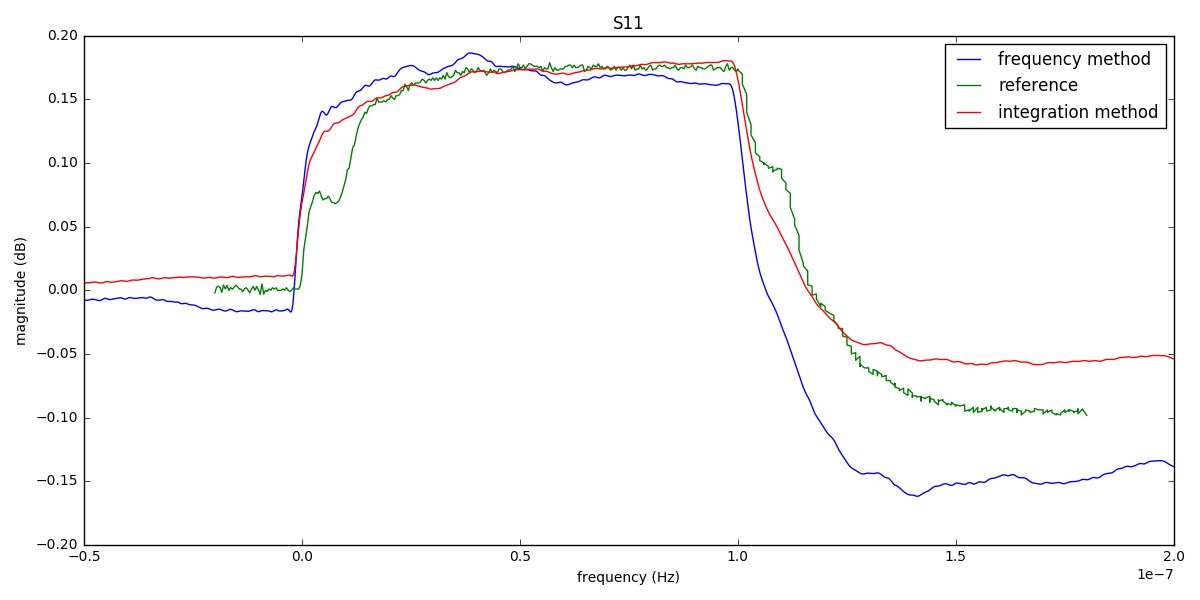
\includegraphics[width=0.9\textwidth]{src/3/figures/final_comparison_reconstructions.png}
  \caption{Reference current waveform versus frequency-domain and time-domain reconstructions}
  \label{fig:freq-domain-reconstructed}
\end{figure}

\subsection{Conclusion}

% Conclusion
The frequency method is more realistic, because it makes less approximations regarding the physical laws and sensor's geometry.
Overall, it is the method selected to process the measurement data in section \ref{sec:test-vehicle-testing}
The remaining sources of error lie in the layout differences between the calibration sensor and the real sensor.
Also, the bandwidth of the calibration equipment might be too small to reproduce high-frequency events..

The integration method can work for short pulses, but accumulates error over time.

% Code repository
Both post-processing methods were implemented in Python language.
The code is freely distributed \cite{nfs-repository} as open-source software under the MIT licensing \cite{mit-licensing}.
